\section{Operation}
\label{chapter2}
\subsection{General}
The SafeSU attaches to a 128-bit wide AHB bus but only supports Single burst 32-bit accesses. AHB Lock accesses and protection control are not implemented.\\
\\
The unit is compatible with GRLIB \textit{plug\&play}(P\&P). Vendor and device's default configuration values are  \textit{"BSC"} and \textit{" AHB Performance Monitoring Unit"} respectively. Regardless, release  \textit{v3.2.4}  of GRMON, the unit may appear as \textit{"Unknown device"}.
\subsection{Default input events}
%explain signals
%distinction bteen CCS and regular signals
In its default implementation, the unit provides up to 256 input events. Each one of the events can be routed to any mechanism of the module through the crossbar.\\
\\
Table \ref{table:t_ev} shows the inputs and mapping to the crossbar input for the current \href{https://gitlab.bsc.es/selene/selene-hardware/-/merge_requests/2}{SELENE release}. The number of signals and arrangements may change in the upcoming versions. \\

\begin{center}
	\begin{longtable}{|l|l|l|l|}
		\caption[SELENE input events. 256 inputs, 6 cores]{SELENE GPL input events. 256 inputs, 6 cores} \label{table:t_ev} \\


		\hline \multicolumn{1}{|c|}{\textbf{Index}} & \multicolumn{1}{c|}{\textbf{Type}}
		& \multicolumn{1}{c|}{\textbf{Source}} & \multicolumn{1}{c|}{\textbf{Description}} \\ \hline
		\endfirsthead

		\multicolumn{3}{c}%
		{{\bfseries \tablename\ \thetable{} -- continued from previous page}} \\
		\hline \multicolumn{1}{|c|}{\textbf{Index}} &
		\multicolumn{1}{c|}{\textbf{Type}} &
		\multicolumn{1}{c|}{\textbf{Source}} &
		\multicolumn{1}{c|}{\textbf{Description}} \\ \hline
		\endhead

		\hline \multicolumn{3}{|r|}{{Continued on next page}} \\ \hline
		\endfoot

		\hline \hline
		\endlastfoot

\hline
0   & Debug   & local  &  Constant HIGH, used for debug purposes or clock cycles \\
1   & Debug   & local  &  Constant LOW, used for debug purposes \\
2   & Pulse   & Core 0 &  Instruction count pipeline 0 \\
3   & Pulse   & Core 0 &  Instruction count pipeline 1 \\
4   & Pulse   & Core 0 &  Instruction cache miss \\
5   & Pulse   & Core 0 &  Instruction TLB miss \\
6   & Pulse   & Core 0 &  Data cache L1 miss \\
7   & Pulse   & Core 0 &  Data TLB miss \\
8   & Pulse   & Core 0 &  Branch predictor miss \\
9   & Pulse   & Core 1 &  Instruction count pipeline 0 \\
10  & Pulse   & Core 1 &  Instruction count pipeline 1 \\
11  & Pulse   & Core 1 &  Instruction cache miss \\
12  & Pulse   & Core 1 &  Instruction TLB miss \\
13  & Pulse   & Core 1 &  Data cache L1 miss \\
14  & Pulse   & Core 1 &  Data TLB miss \\
15  & Pulse   & Core 1 &  Branch predictor miss \\
16  & Pulse   & Core 2 &  Instruction count pipeline 0 \\
17  & Pulse   & Core 2 &  Instruction count pipeline 1 \\
18  & Pulse   & Core 2 &  Instruction cache miss \\
19  & Pulse   & Core 2 &  Instruction TLB miss \\
20  & Pulse   & Core 2 &  Data cache L1 miss \\
21  & Pulse   & Core 2 &  Data TLB miss \\
22  & Pulse   & Core 2 &  Branch predictor miss \\
23  & Pulse   & Core 3 &  Instruction count pipeline 0 \\
24  & Pulse   & Core 3 &  Instruction count pipeline 1 \\
25  & Pulse   & Core 3 &  Instruction cache miss \\
26  & Pulse   & Core 3 &  Instruction TLB miss \\
27  & Pulse   & Core 3 &  Data cache L1 miss \\
28  & Pulse   & Core 3 &  Data TLB miss \\
29  & Pulse   & Core 3 &  Branch predictor miss \\
30  & Pulse   & Core 4 &  Instruction count pipeline 0 \\
31  & Pulse   & Core 4 &  Instruction count pipeline 1 \\
32  & Pulse   & Core 4 &  Instruction cache miss \\
33  & Pulse   & Core 4 &  Instruction TLB miss \\
34  & Pulse   & Core 4 &  Data cache L1 miss \\
35  & Pulse   & Core 4 &  Data TLB miss \\
36  & Pulse   & Core 4 &  Branch predictor miss \\
37  & Pulse   & Core 5 &  Instruction count pipeline 0 \\
38  & Pulse   & Core 5 &  Instruction count pipeline 1 \\
39  & Pulse   & Core 5 &  Instruction cache miss \\
40  & Pulse   & Core 5 &  Instruction TLB miss \\
41  & Pulse   & Core 5 &  Data cache L1 miss \\
42  & Pulse   & Core 5 &  Data TLB miss \\
43  & Pulse   & Core 5 &  Branch predictor miss \\
44  & CCS AHB &  -     &  Agressor C1 Victim C0\\
45  & CCS AHB &  -     &  Agressor C2 Victim C0\\
46  & CCS AHB &  -     &  Agressor C3 Victim C0\\
47  & CCS AHB &  -     &  Agressor C4 Victim C0\\
48  & CCS AHB &  -     &  Agressor C5 Victim C0\\
49  & CCS AHB &  -     &  Agressor C0 Victim C1\\
50  & CCS AHB &  -     &  Agressor C2 Victim C1\\
51  & CCS AHB &  -     &  Agressor C3 Victim C1\\
52  & CCS AHB &  -     &  Agressor C4 Victim C1\\
53  & CCS AHB &  -     &  Agressor C5 Victim C1\\
54  & CCS AHB &  -     &  Agressor C0 Victim C2\\
55  & CCS AHB &  -     &  Agressor C1 Victim C2\\
56  & CCS AHB &  -     &  Agressor C3 Victim C2\\
57  & CCS AHB &  -     &  Agressor C4 Victim C2\\
58  & CCS AHB &  -     &  Agressor C5 Victim C2\\
59  & CCS AHB &  -     &  Agressor C0 Victim C3\\
60  & CCS AHB &  -     &  Agressor C1 Victim C3\\
61  & CCS AHB &  -     &  Agressor C2 Victim C3\\
62  & CCS AHB &  -     &  Agressor C4 Victim C3\\
63  & CCS AHB &  -     &  Agressor C5 Victim C3\\
64  & CCS AHB &  -     &  Agressor C0 Victim C4\\
65  & CCS AHB &  -     &  Agressor C1 Victim C4\\
66  & CCS AHB &  -     &  Agressor C2 Victim C4\\
67  & CCS AHB &  -     &  Agressor C3 Victim C4\\
68  & CCS AHB &  -     &  Agressor C5 Victim C4\\
69  & CCS AHB &  -     &  Agressor C0 Victim C5\\
70  & CCS AHB &  -     &  Agressor C1 Victim C5\\
71  & CCS AHB &  -     &  Agressor C2 Victim C5\\
72  & CCS AHB &  -     &  Agressor C3 Victim C5\\
73  & CCS AHB &  -     &  Agressor C4 Victim C5\\
74  & CSS AXI &  -     &  MLKEM0 write length -- 1 beat(4-byte)\\
75  & CSS AXI &  -     &  MLKEM0 write length -- 4 beat(16-byte)\\
76  & CSS AXI &  -     &  MLKEM0 read  length -- 1 beat(16-byte)\\
77  & CSS AXI &  -     &  MLKEM0 read  length -- 2 beat(16-byte)\\
78  & CSS AXI &  -     &  MLKEM0 read  length -- 3 beat(16-byte)\\
79  & CSS AXI &  -     &  MLKEM0 read  length -- 4 beat(16-byte)\\
80  & CSS AXI &  -     &  MLKEM0 read  length -- 5 beat(16-byte)\\
81  & CSS AXI &  -     &  MLKEM1 write length -- 2 beat(16-byte)\\
82  & CSS AXI &  -     &  MLKEM1 write length -- 4 beat(16-byte)\\
83  & CSS AXI &  -     &  MLKEM2 read  length -- 1 beat(16-byte)\\
84  & CSS AXI &  -     &  MLKEM2 read  length -- 2 beat(16-byte)\\
85  & CSS AXI &  -     &  MLKEM2 read  length -- 3 beat(16-byte)\\
86  & CSS AXI &  -     &  MLKEM2 read  length -- 4 beat(16-byte)\\
87  & CSS AXI &  -     &  MLKEM2 read  length -- 5 beat(16-byte)\\
88  & CSS AXI &  -     &  MLKEM3 read  length -- 1 beat(16-byte)\\
89  & CSS AXI &  -     &  MLKEM3 read  length -- 2 beat(16-byte)\\
90  & CSS AXI &  -     &  MLKEM3 read  length -- 3 beat(16-byte)\\
91  & CSS AXI &  -     &  MLKEM3 read  length -- 4 beat(16-byte)\\
92  & CSS AXI &  -     &  MLKEM3 read  length -- 5 beat(16-byte)\\
93  & CSS AXI &  -     &  MLKEM4 read  length -- 1 beat(16-byte)\\
94  & CSS AXI &  -     &  MLKEM4 read  length -- 2 beat(16-byte)\\
95  & CSS AXI &  -     &  MLKEM4 read  length -- 3 beat(16-byte)\\
96  & CSS AXI &  -     &  MLKEM4 read  length -- 4 beat(16-byte)\\
97  & CSS AXI &  -     &  MLKEM4 read  length -- 5 beat(16-byte)\\
98  & CSS AXI &  -     &  MLDSA0 write length -- 1 beat(4-byte)\\
99  & CSS AXI &  -     &  MLDSA0 write length -- 2 beat(16-byte)\\
100 & CSS AXI &  -     &  MLDSA0 write length -- 4 beat(16-byte)\\
101 & CSS AXI &  -     &  MLDSA1 write length -- 4 beat(16-byte)\\
102 & CSS AXI &  -     &  MLDSA1 read  length -- 1 beat(16-byte)\\
103 & CSS AXI &  -     &  MLDSA1 read  length -- 2 beat(16-byte)\\
104 & CSS AXI &  -     &  MLDSA1 read  length -- 3 beat(16-byte)\\
105 & CSS AXI &  -     &  MLDSA1 read  length -- 4 beat(16-byte)\\
106 & CSS AXI &  -     &  MLDSA1 read  length -- 5 beat(16-byte)\\
107 & CSS AXI &  -     &  MLDSA2 read  length -- 3 beat(16-byte)\\
108 & CSS AXI &  -     &  MLDSA2 read  length -- 4 beat(16-byte)\\
109 & CSS AXI &  -     &  MLDSA2 read  length -- 5 beat(16-byte)\\
110 & CSS AXI &  -     &  MLDSA3 read  length -- 1 beat(16-byte)\\
111 & CSS AXI &  -     &  MLDSA3 read  length -- 2 beat(16-byte)\\
112 & CSS AXI &  -     &  MLDSA3 read  length -- 3 beat(16-byte)\\
113 & CSS AXI &  -     &  MLDSA3 read  length -- 4 beat(16-byte)\\
114 & CSS AXI &  -     &  MLDSA3 read  length -- 5 beat(16-byte)\\
115 & CSS AXI &  -     &  MLDSA4 read  length -- 1 beat(16-byte)\\
116 & CSS AXI &  -     &  MLDSA4 read  length -- 2 beat(16-byte)\\
117 & CSS AXI &  -     &  MLDSA4 read  length -- 3 beat(16-byte)\\
118 & CSS AXI &  -     &  MLDSA4 read  length -- 4 beat(16-byte)\\
119 & CSS AXI &  -     &  MLDSA4 read  length -- 5 beat(16-byte)\\
120 & - & - &   Filler signal, constant 0 \\
... & - & - &   Filler signal, constant 0 \\
241 & - & - &   Filler signal, constant 0 \\
242 & CCS AHB & - &   Aggressor others Victim C0 \\
243 & - & - &   Filler signal, constant 0 \\
244 & - & - &   Filler signal, constant 0 \\
245 & - & - &   Filler signal, constant 0 \\
246 & - & - &   Filler signal, constant 0 \\
247 & - & - &   Filler signal, constant 0 \\
248 & CCS AHB & - &   Generic, Aggressor 0 Victim 0\\
249 & CCS AHB & - &   Generic, Aggressor 1 Victim 0 \\
250 & CCS AHB & - &   Generic, Aggressor 2 Victim 0 \\
251 & CCS AHB & - &   Generic, Aggressor 3 Victim 0 \\
252 & CCS AHB & - &   Generic, Aggressor 4 Victim 0 \\
253 & CCS AHB & - &   Generic, Aggressor 5 Victim 0 \\
254 & CCS AHB & - &   Residual, Victim 0  \\
255 & - & - &   Filler signal, constant 0 \\
	\end{longtable}
\end{center}

\begin{table}[H]
	\caption{Mapping from Master qos (MQ) to IPs on GPL release. }
	\label{table:t_ev2}
	\centering
		\begin{tabular}{|l|l|l|l|l|}
			\hline
			\textbf{MQ} & \textbf{Bus of origin}  & \textbf{Bus ID} & \textbf{Description}\\
			\hline
0 & AHB & 0 &  NOEL-V CORE \\
1 & AHB & 1 &  NOEL-V CORE \\
2 & AHB & 2 &  NOEL-V CORE \\
3 & AHB & 3 &  NOEL-V CORE \\
4 & AHB & 4 &  NOEL-V CORE \\
5 & AHB & 5 &  NOEL-V CORE \\
6 & AHB & 6 &  GR Ethernet MAC \\
7 & AHB & 7 &  GRDMAC2 DMA Controller \\
8 & AHB & 8 &  AHB Debug UART \\
9 & AHB & 9 &  JTAG Debug Link \\
10 & AHB & 10 &  EDCL master interface   \\
11 & - & - & Unused \\
12 & - & - & Unused  \\
13 & - & - & Unused   \\
14 & - & - & Unused  \\
	\hline
		\end{tabular}
\end{table}

\begin{table}[H]
	\caption{Maping from Master qos (MQ) to IPs on non-GPL release}
	\label{table:t_ev3}
	\centering
	\begin{tabular}{|l|l|l|l|l|}
		\hline
		\textbf{MQ} & \textbf{Bus of origin}  & \textbf{Bus ID} & \textbf{Description}\\
		\hline
0 & AHB & 0 &  NOEL-V CORE \\
1 & AHB & 1 &  NOEL-V CORE \\
2 & AHB & 2 &  NOEL-V CORE \\
3 & AHB & 3 &  NOEL-V CORE \\
4 & AHB & 4 &  NOEL-V CORE \\
5 & AHB & 5 &  NOEL-V CORE \\

6 & AHB & 6 &  GR Ethernet MAC \\
7 & AHB & 7 &  GRSPW2 SpaceWire \\
8 & AHB & 8 &  GRSPW2 SpaceWire \\
9 & AHB & 9 &  CAN-FD Controller with DMA \\
10 & AHB & 10 &  CAN-FD Controller with DMA \\
11 & AHB & 11 & GRDMAC2 DMA Controller \\
12 & AHB & 12 & AHB Debug UART  \\
13 & AHB & 13 & JTAG Debug Link   \\
14 & AHB & 14 & EDCL master interface  \\
	\hline
	\end{tabular}
\end{table}
Signals labeled as \textit{debug} are fix inputs that can be used to test hardware or software with known inputs. \textbf{Event 0} (fix '1') can be used to measure the \textbf{number of elapsed cycles}.\\
\\
Signals of type \textit{CCS} can be used to compute the total contention cycle stack of the system. These signals become high at the first rising edge of the clock after a given condition or event has been detected. They remain active until the condition or event that they are measuring becomes low. This behavior allows measuring the length of clock cycles. When generating CCS signals, the user must consider if they want to allow back to back events and generate the input signals accordingly at RTL level.

The generic and residual contention metrics have the following meanings:
\begin{itemize}
\item \textbf{Generic contention}: The previous request has been served, but has left the slave in an unready state, making this core's request be delayed this cycle. We assume that the slave would be ready if the previous master had not accessed it.
\item \textbf{Residual contention}: We observed that, when using the gaisler L2-lite cache, if a htrans "10"(NONSEQ) happens after a non-idle transaction, the response to the current master (the one that issued the "10") transaction is delayed by one cycle. THIS IS GAISLER L2 LITE specific, thus, not portable
\end{itemize}


\subsection{Main configuration and self-test}
Reset and enable of overflow and regular counters can be performed with register \ref{base_cfg}. All signals are active high.\\
Self-test mode allows to bypass the input events from the crossbar and instead use a specific input pattern where signals are constant. This mode can be used for debugging. After the addition of the crossbar and debug inputs, there is a certain overlap. The same results can be achieved with the correct crossbar configuration. Nevertheless, it has been included in this release for compatibility.\\
\\
These are the Self-test modes for each configuration value of the fied \textit{selftest mode} in register \ref{base_cfg}:
\begin{itemize}
	\item 0b00: Events depend on the crossbar. Self-test is disabled
	\item 0b01: All signals are set to 1.
	\item 0b10: All signals are set to 0.
	\item 0b11: Signal 0 is set to 1.  The remaining signals are set to 0.
\end{itemize}

 \begin{register}{H}{Base configuration register}{0x000}
   \label{base_cfg}
   \regfield{Selftest mode}{2}{30}{{00}}
   \regfield{Reserved}{24}{5}{x}
   \regfield{Overflow softreset}{1}{3}{0}
   \regfield{Overflow enable}{1}{2}{0}
   \regfield{General Softreset}{1}{1}{0}
   \regfield{General Enable}{1}{0}{0}
   \reglabel{Reset value}\regnewline
  \end{register}

\subsection{Crossbar}
This feature allows routing any of the input signals of table \ref{table:t_ev} or \ref{table:t_ev2} into any of the 24 counters of the SafeSU. Each one of the counters has a 5-bit configuration value for the 32 input version of the crossbar, 7-bit for the 128 version and 8-bit for the 256 version. For simplicity this section describes the 32 entry variant of the crossabar. Consider that the width of the configuration field is $log2(N\_inputs)$ and the total amount of configuration registers $log2(N\_inputs)*N\_inputs$.\\
Configuration values are stored in registers \ref{cross_cfg0}, \ref{cross_cfg1}, \ref{cross_cfg2},\ref{cross_cfg3}. All the configuration values are consecutive. Thus some values may have configuration bits in two consecutive memory addresses. Examples of this are Output 6, 12, 19 in our current configuration. As a consequence, the previous outputs may require two writes to configure the desired input signal.\\
\\
Configuration fields match one to one with the internal counters. So the field \textit{output 0} matches with \textit{counter 0}, \textit{output 1} with\textit{ counter 1} and so on.\\
\\
As a usage example, suppose the user wants to route the signal \textit{pmu\_events(0).icnt(0)} to the internal \textit{counter 0}. The field \textit{Output 0} of register \ref{cross_cfg0} shall match the  Index of the signal in table \ref{table:t_ev}. In this case, the index is 2. After this configuration, the event count will be recorded in \textit{counter 0}. The addresses for counter values are indicated in figure \ref{fig:counters0}.\\
\\
 \begin{register}{H}{Crossbar configuration register 0}{0x0AC}
	\label{cross_cfg0}
	\regfield{Output 6 [1:0]}{2}{30}{{00}}
	\regfield{Output 5}{5}{25}{{00}}
	\regfield{Output 4}{5}{20}{{00}}
	\regfield{Output 3}{5}{15}{{00}}
	\regfield{Output 2}{5}{10}{{00}}
	\regfield{Output 1}{5}{5}{{00}}
	\regfield{Output 0}{5}{0}{{00}}
	\reglabel{Reset value}\regnewline

\end{register}

 \begin{register}{H}{Crossbar configuration register 1}{0x0B0}
	\label{cross_cfg1}
	\regfield{Output 12[3:0]}{4}{28}{{00}}
	\regfield{Output 11}{5}{23}{{00}}
	\regfield{Output 10}{5}{18}{{00}}
	\regfield{Output 9}{5}{13}{{00}}
	\regfield{Output 8}{5}{8}{{00}}
	\regfield{Output 7}{5}{3}{{00}}
	\regfield{Output 6 [4:2]}{3}{0}{{00}}
	\reglabel{Reset value}\regnewline
\end{register}

 \begin{register}{H}{Crossbar configuration register 2}{0x0B4}
	\label{cross_cfg2}
	\regfield{Output 19 [0:0]}{1}{31}{{00}}
	\regfield{Output 18}{5}{26}{{00}}
	\regfield{Output 17}{5}{21}{{00}}
	\regfield{Output 16}{5}{16}{{00}}
	\regfield{Output 15}{5}{11}{{00}}
	\regfield{Output 14}{5}{6}{{00}}
	\regfield{Output 13}{5}{1}{{00}}
	\regfield{Output 12[4:4]}{1}{0}{{00}}
	\reglabel{Reset value}\regnewline
\end{register}

 \begin{register}{H}{Crossbar configuration register 3}{0x0B8}
	\label{cross_cfg3}
	\regfield{Reserved}{3}{29}{{x}}
	\regfield{Output 24}{5}{24}{{00}}
	\regfield{Output 23}{5}{19}{{00}}
	\regfield{Output 22}{5}{14}{{00}}
	\regfield{Output 21}{5}{9}{{00}}
	\regfield{Output 20}{5}{4}{{00}}
	\regfield{Output 19[4:1]}{4}{0}{{00}}
	\reglabel{Reset value}\regnewline
\end{register}
Signal routing is important since some of the SafeSU features are only available at different crossbar outputs. Table \ref{tab:features} shows the available capabilities for each one of the outputs\footnotetext{RDC and MCCU signals are only available if the assigned core is synthesized.}.\\
\begin{table}
	\caption{Crossbar outputs and SafeSU capabilities}
	\label{tab:features}
\begin{small}
	\begin{center}
		\begin{tabular}{|l|l|l|l|l|l|}
			\hline
			\textbf{Output} & \textbf{Counters} & \textbf{Overflow}  & \textbf{MCCU}  & \textbf{RDC} & \textbf{ALT MCCU}\\
			\hline
			0 & Yes & Yes & Core 0 & Yes & No \\
			\hline
			1 & Yes & Yes & Core 0 & Yes & No \\
			\hline
			2 & Yes & Yes & Core 1 & Yes & No \\
			\hline
			3 & Yes & Yes & Core 1 & Yes & No \\
			\hline
			4 & Yes & Yes & Core 2 & Yes & No \\
			\hline
			5 & Yes & Yes & Core 2 & Yes & No \\
			\hline
			6 & Yes & Yes & Core 3 & Yes & No \\
			\hline
			7 & Yes & Yes & Core 3 & Yes & No \\
			\hline
			8 & Yes & Yes & Core 4 & Yes & Yes \\
			\hline
			9 & Yes & Yes & Core 4 & Yes & Yes \\
			\hline
			10 & Yes & Yes & Core 5 & Yes & Yes \\
			\hline
			11 & Yes & Yes & Core 5 & Yes & Yes \\
			\hline
			12 & Yes & Yes & No & No & Yes \\
			\hline
			13 & Yes & Yes & No & No & Yes \\
			\hline
			14 & Yes & Yes & No & No & Yes \\
			\hline
			15 & Yes & Yes & No & No & Yes \\
			\hline
			16 & Yes & Yes & No & No & Yes \\
			\hline
			17 & Yes & Yes & No & No & Yes \\
			\hline
			18 & Yes & Yes & No & No & Yes \\
			\hline
			19 & Yes & Yes & No & No & Yes \\
			\hline
			20 & Yes & Yes & No & No & Yes \\
			\hline
			21 & Yes & Yes & No & No & Yes \\
			\hline
			22 & Yes & Yes & No & No & Yes \\
			\hline
			23 & Yes & Yes & No & No & Yes \\
			\hline
		\end{tabular}
	\end{center}
\end{small}
\end{table}

\subsection{Counters}\label{sec:count}
The unit in the default configuration contains 24 counters, 32-bit each. Figures \ref{fig:counters0} and \ref{fig:counters1} indicate the memory address where each counter's value can be access. Counter values can be \textbf{read} or \textbf{written}, thus allowing to set the initial value of the counters.\\
\\
Enable and reset is managed by the base configuration register \ref{base_cfg}.\\
\\
Counters can overflow. In such a case, the count will wrap back to 0 and keep counting. Section \ref{sec:over} describes how to enable the overflow detection interrupts.\\
\\
\begin{figure}[H]
	\begin{center}
		\regfieldb{0x04}{32}{0}
		\reglabelb{Counter 0} \\
		\regfieldb{0x08}{32}{0}
		\reglabelb{Counter 1} \\
		\regfieldb{0x0C}{32}{0}
		\reglabelb{Counter 2} \\
		\regfieldb{0x10}{32}{0}
		\reglabelb{Counter 3} \\
		\regfieldb{0x14}{32}{0}
		\reglabelb{Counter 4} \\
		\regfieldb{0x18}{32}{0}
		\reglabelb{Counter 5} \\
		\regfieldb{0x1C}{32}{0}
		\reglabelb{Counter 6} \\
		\regfieldb{0x20}{32}{0}
		\reglabelb{Counter 7} \\
		\regfieldb{0x24}{32}{0}
		\reglabelb{Counter 8} \\
		\regfieldb{0x28}{32}{0}
		\reglabelb{Counter 9} \\
		\regfieldb{0x2C}{32}{0}
		\reglabelb{Counter 10} \\
		\regfieldb{0x30}{32}{0}
		\reglabelb{Counter 11} \\
		\regfieldb{0x34}{32}{0}
		\reglabelb{Counter 12} \\
		\end{center}
	\caption{0 to 12 Counter adresses}\label{fig:counters0}
\end{figure}

\begin{figure}[H]
	\begin{center}
		\regfieldb{0x38}{32}{0}
		\reglabelb{Counter 13} \\
		\regfieldb{0x3C}{32}{0}
		\reglabelb{Counter 14} \\
		\regfieldb{0x40}{32}{0}
		\reglabelb{Counter 15} \\
		\regfieldb{0x44}{32}{0}
		\reglabelb{Counter 16} \\
		\regfieldb{0x48}{32}{0}
		\reglabelb{Counter 17} \\
		\regfieldb{0x4C}{32}{0}
		\reglabelb{Counter 18} \\
		\regfieldb{0x50}{32}{0}
		\reglabelb{Counter 19} \\
		\regfieldb{0x54}{32}{0}
		\reglabelb{Counter 20} \\
		\regfieldb{0x58}{32}{0}
		\reglabelb{Counter 21} \\
		\regfieldb{0x5C}{32}{0}
		\reglabelb{Counter 22} \\
		\regfieldb{0x60}{32}{0}
		\reglabelb{Counter 23} \\
	\end{center}
	\caption{12 to 24 Counter addresses}\label{fig:counters1}
\end{figure}

\subsection{Overflow}
\label{sec:over}
The user can enable overflow detection for each one of the counters in section \ref{sec:count}. Enables are active high and individual for each counter, as indicated in register \ref{reg:over_cfg0}. If a counter with overflow detection active wraps over the maximum value, the corresponding bit of register \ref{reg:over_itrv} will become 1, and  AHB interrupt number 6 will become active.\\
\\
The default AHB interrupt mapping can be modified within the file \textit{ahb\_wrapper.vhd}.
\begin{register}{H}{Overflow interrupt enable mask}{0x064}
	\begin{tiny}
		\label{reg:over_cfg0}
		\regfield{Reserved}{8}{24}{{x}}
		\regfield{Counter 23}{1}{23}{{0}}
		\regfield{Counter 22}{1}{22}{{0}}
		\regfield{Counter 21}{1}{21}{{0}}
		\regfield{Counter 20}{1}{20}{{0}}
		\regfield{Counter 19}{1}{19}{{0}}
		\regfield{Counter 18}{1}{18}{{0}}
		\regfield{Counter 17}{1}{17}{{0}}
		\regfield{Counter 16}{1}{16}{{0}}
		\regfield{Counter 15}{1}{15}{{0}}
		\regfield{Counter 14}{1}{14}{{0}}
		\regfield{Counter 13}{1}{13}{{0}}
		\regfield{Counter 12}{1}{12}{{0}}
		\regfield{Counter 11}{1}{11}{{0}}
		\regfield{Counter 10}{1}{10}{{0}}
		\regfield{Counter 9}{1}{9}{{0}}
		\regfield{Counter 8}{1}{8}{{0}}
		\regfield{Counter 7}{1}{7}{{0}}
		\regfield{Counter 6}{1}{6}{{0}}
		\regfield{Counter 5}{1}{5}{{0}}
		\regfield{Counter 4}{1}{4}{{0}}
		\regfield{Counter 3}{1}{3}{{0}}
		\regfield{Counter 2}{1}{2}{{0}}
		\regfield{Counter 1}{1}{1}{{0}}
		\regfield{Counter 0}{1}{0}{{0}}
		\reglabel{Reset value}\regnewline
	\end{tiny}
\end{register}

\begin{register}{H}{Overflow interrupt vector }{0x068}
	\label{reg:over_itrv}
	\begin{tiny}
		\regfield{Reserved}{8}{24}{{0}}
		\regfield{Counter 23}{1}{23}{{0}}
		\regfield{Counter 22}{1}{22}{{0}}
		\regfield{Counter 21}{1}{21}{{0}}
		\regfield{Counter 20}{1}{20}{{0}}
		\regfield{Counter 19}{1}{19}{{0}}
		\regfield{Counter 18}{1}{18}{{0}}
		\regfield{Counter 17}{1}{17}{{0}}
		\regfield{Counter 16}{1}{16}{{0}}
		\regfield{Counter 15}{1}{15}{{0}}
		\regfield{Counter 14}{1}{14}{{0}}
		\regfield{Counter 13}{1}{13}{{0}}
		\regfield{Counter 12}{1}{12}{{0}}
		\regfield{Counter 11}{1}{11}{{0}}
		\regfield{Counter 10}{1}{10}{{0}}
		\regfield{Counter 9}{1}{9}{{0}}
		\regfield{Counter 8}{1}{8}{{0}}
		\regfield{Counter 7}{1}{7}{{0}}
		\regfield{Counter 6}{1}{6}{{0}}
		\regfield{Counter 5}{1}{5}{{0}}
		\regfield{Counter 4}{1}{4}{{0}}
		\regfield{Counter 3}{1}{3}{{0}}
		\regfield{Counter 2}{1}{2}{{0}}
		\regfield{Counter 1}{1}{1}{{0}}
		\regfield{Counter 0}{1}{0}{{0}}
		\reglabel{Reset value}\regnewline
	\end{tiny}
\end{register}

\subsection{MCCU}
The Maximum-Contention Control Unit (MCCU) allows to monitor a subset of the input events and track the approximate contention that they will cause. Currently, events assigned to counters 0 to 11 can be used as inputs of the MCCU. Thanks to the crossbar, any of the SoC signals can be used by the MCCU. In this section we use the 4 core version as a reference. In all configurations one quota register is assigned to each core and one weight is asigned to each signal.\\
\\
\begin{figure}[H]
	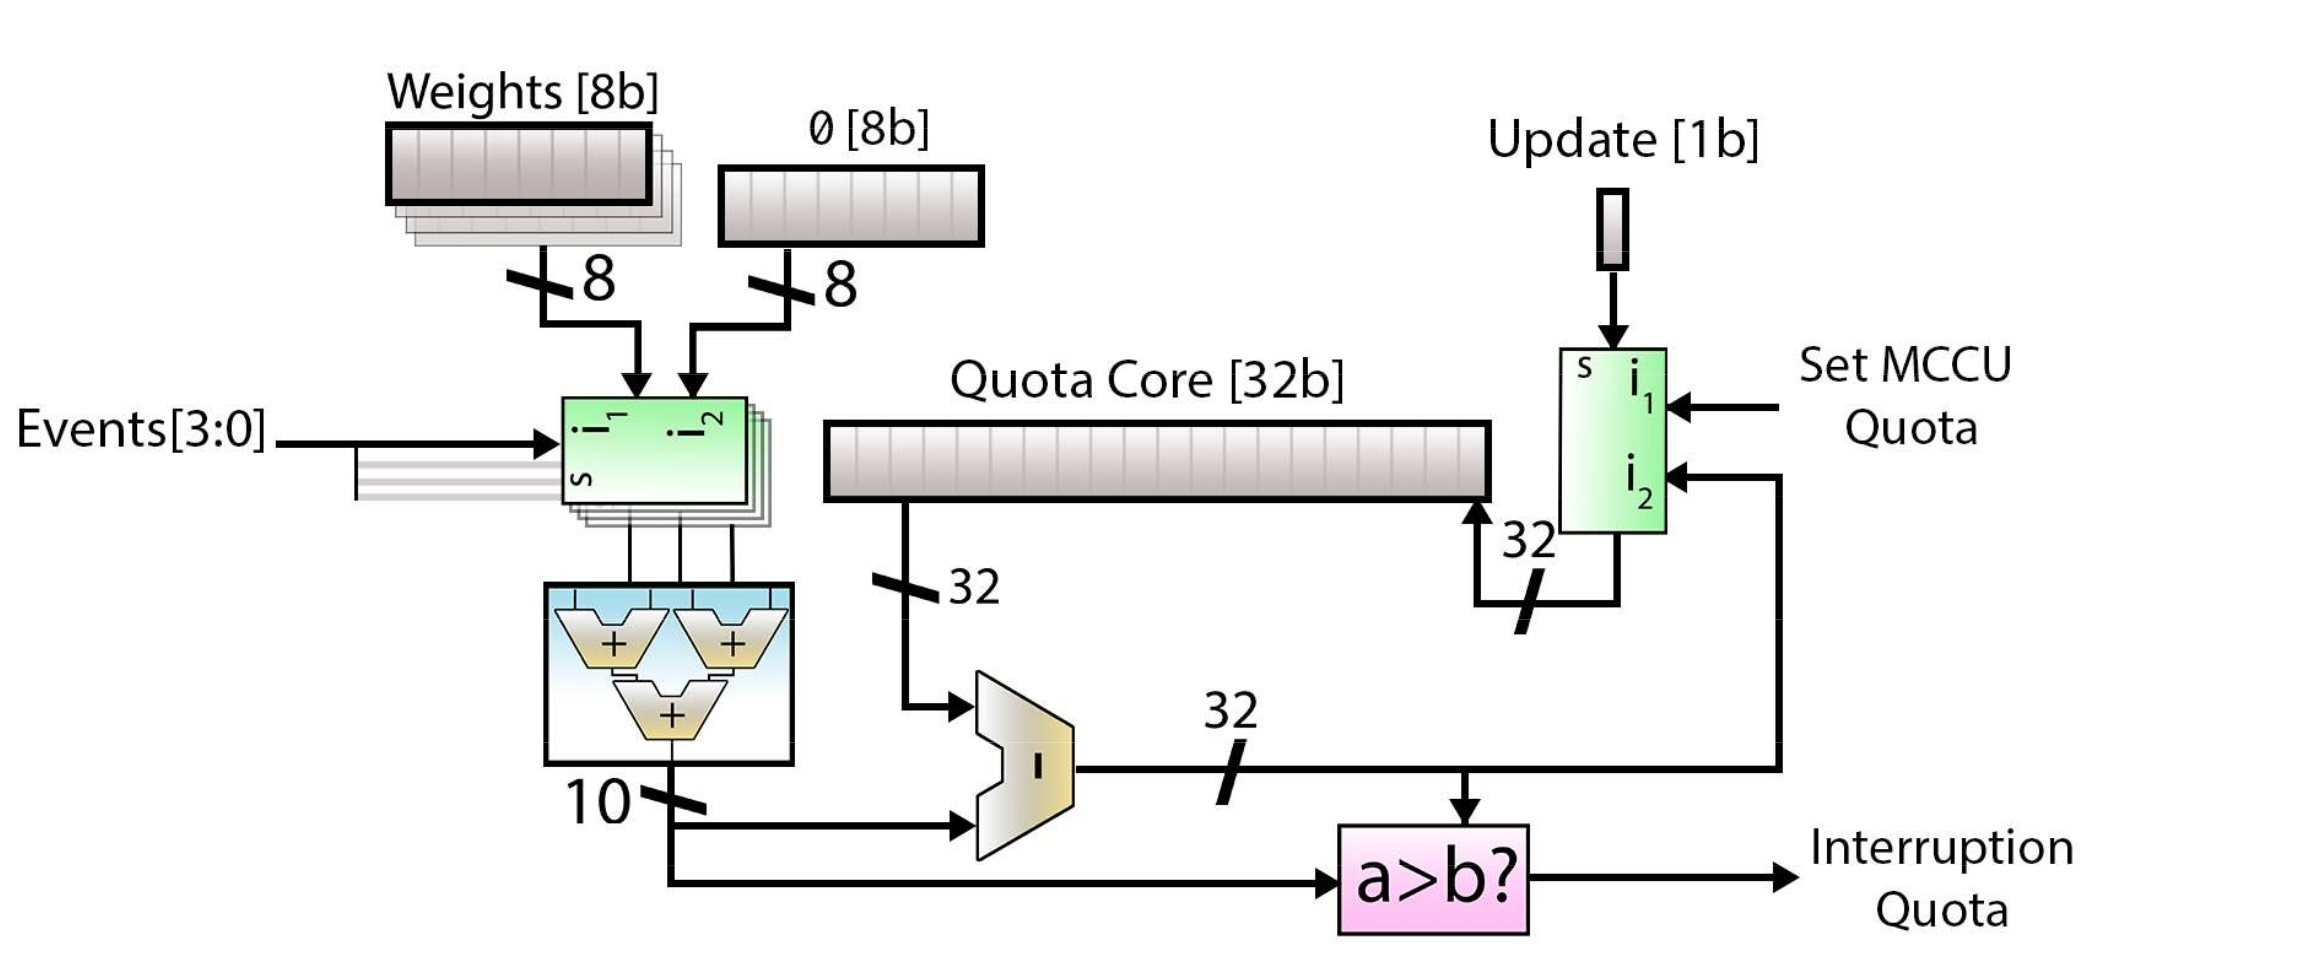
\includegraphics[keepaspectratio,width=\columnwidth]{img/bd_MCCU.png}
	\caption{Block diagram MCCU mechanism for one core.}
	\label{fig:blk_MCCU}
\end{figure}
Figure \ref{fig:blk_MCCU} shows the internal elements required to monitor the quota consumption of one core, given four input events.  When events are active, they pass the value assigned in the weight register \ref{MCCU_weight0} for the given signal to a series of adders. The addition is subtracted from the corresponding quota register \ref{fig:MCCU_ava}. When the remaining quota is smaller than the cycle contention, an interrupt is triggered.

When the "Enable Hardware Quota" bit is toggled, this interrupt is routed to the AHB controller directly to block contending core access to the shared bus. Thus, disabling the interrupt lines and performing the decisions without software intervention.


\begin{register}{}{MCCU main configuration for 6 core configurations}{0x074}
	\label{MCCU_cfg_6c}
	\regfield{Enable Hardware Quota}{1}{31}{{0}}
	\regfield{Reserved}{18}{13}{{x}}
	\regfield{Soft reset RDC}{1}{12}{{0}}
	\regfield{Enable RDC}{1}{11}{{0}}
	\regfield{Update Quota PQC Write}{1}{10}{{0}}
	\regfield{Update Quota PQC Read}{1}{9}{{0}}
	\regfield{Update Quota PQC Read \& Write}{1}{8}{{0}}
	\regfield{Update Quota Core 5}{1}{7}{{0}}
	\regfield{Update Quota Core 4}{1}{6}{{0}}
	\regfield{Update Quota Core 3}{1}{5}{{0}}
	\regfield{Update Quota Core 2}{1}{4}{{0}}
	\regfield{Update Quota Core 1}{1}{3}{{0}}
	\regfield{Update Quota Core 0}{1}{2}{{0}}
	\regfield{Soft reset MCCU}{1}{1}{{0}}
	\regfield{Enable reset MCCU}{1}{0}{{0}}
	\reglabel{Reset value}\regnewline
\end{register}
\begin{figure}[H]
	\begin{center}
		\regfieldb{0x078}{32}{0}
		\reglabelb{Core 0} \\
		\regfieldb{0x07c}{32}{0}
		\reglabelb{Core 1} \\
		\regfieldb{0x080}{32}{0}
		\reglabelb{Core 2} \\
		\regfieldb{0x084}{32}{0}
		\reglabelb{Core 3} \\
		\regfieldb{0x088}{32}{0}
		\reglabelb{Core 4} \\
		\regfieldb{0x08C}{32}{0}
		\reglabelb{Core 5} \\
	\end{center}
	\caption{MCCU Quota limits for each core}\label{fig:MCCU_lim}
\end{figure}
\begin{figure}[H]
	\begin{center}
		\regfieldb{0x09C}{32}{0}
		\reglabelb{Core 0} \\
		\regfieldb{0x0A0}{32}{0}
		\reglabelb{Core 1} \\
		\regfieldb{0x0A4}{32}{0}
		\reglabelb{Core 2} \\
		\regfieldb{0x0A8}{32}{0}
		\reglabelb{Core 3} \\
		\regfieldb{0x0Ac}{32}{0}
		\reglabelb{Core 4} \\
		\regfieldb{0x0B0}{32}{0}
		\reglabelb{Core 5} \\
	\end{center}
	\caption{MCCU Current remaining Quota for each core}\label{fig:MCCU_ava}
\end{figure}
In the current release, the MCCU can be reset and activated with the respective fields of register \ref{MCCU_cfg_6c}. The fields labeled as \textit{Update Quota core} are used to update the available quota of each core (figure \ref{fig:MCCU_ava}). While  \textit{Update Quota core} is high, the content is assigned to the available quota. Once released (low), the available quota can start to decrease if the MCCU is active. The current quota can be read while the unit is active.\\
\\
In the current release, each core can monitor two input events. The MCCU module is parametric and more events can be provided in future releases.  Table \ref{tab:features} shows the features available for each crossbar output. Under the column MCCU, you can see towards which core quota the event will be computed.
The unit provides one interruption for each of the monitored cores.
%Quota exhaustion for cores 3, 2, 1, and 0 is mapped to AHB interrupts 10, 9, 8, and 7, respectively.\\ it changes across bitstreams
\\
Weights for each monitored event are registered in registers \ref{MCCU_weight0} and \ref{MCCU_weight1}. Currently, each weight is an 8-bit field. Each input of the MCCU maps directly to the outputs of the crossbar. Thus the weight for the MCCU input 0 corresponds to the signal in crossbar output 0.\\
\\
\begin{register}{H}{MCCU event weights register 0 (shared with RDC)}{0x0C0}
	\label{MCCU_weight0}
	\regfield{Input 3}{8}{24}{{00}}
	\regfield{Input 2}{8}{16}{{00}}
	\regfield{Input 1}{8}{8}{{00}}
	\regfield{Input 0}{8}{0}{{00}}
	\reglabel{Reset value}\regnewline
\end{register}
\begin{register}{H}{MCCU event weights register 1 (shared with RDC)}{0x0C4}
	\label{MCCU_weight1}
	\regfield{Input 7}{8}{24}{{00}}
	\regfield{Input 6}{8}{16}{{00}}
	\regfield{Input 5}{8}{8}{{00}}
	\regfield{Input 4}{8}{0}{{00}}
	\reglabel{Reset value}\regnewline
\end{register}
\begin{register}{H}{MCCU event weights register 2 (shared with RDC)}{0x0C8}
	\label{MCCU_weight2}
	\regfield{Input 11}{8}{24}{{00}}
	\regfield{Input 10}{8}{16}{{00}}
	\regfield{Input 9}{8}{8}{{00}}
	\regfield{Input 8}{8}{0}{{00}}
	\reglabel{Reset value}\regnewline
\end{register}

\subsection{Alternative MCCU}
PQC accelerator monitoring is supported by the SafeSU using a secondary MCCU.\\
This implementation differs from the original MCCU in that the input event signals from the crossbar, and weights in a particular interconnection, are shared among 3 additional PQC cores, Read \& Write, Read, and Write cores.

The event signals must be arranged from the crossbar output following a specific order (indexed by the output Crossbar ID) specified by the alternative MCCU hardware implementation.
These are summarized by the particular PQC benchmark configurations, including MLKEM encapsulation (table~\ref{table:t_enc}), MLKEM decapsulation (table~\ref{table:t_decap}), MLDSA signature (table~\ref{table:t_sign}), and MLDSA verification (table~\ref{table:t_ver}).
\begin{table}[H]
	\caption{Counter Assignment for MLKEM Encapsulation. }
	\label{table:t_enc}
	\centering
		\begin{tabular}{|l|l|l|}
			\hline
			\textbf{Event ID} & \textbf{Crossbar ID} & \textbf{Description}\\
			\hline

74  & 8  & MLKEM0 write length -- 1 beat(4-byte)  \\
81  & 9  & MLKEM1 write length -- 2 beat(16-byte) \\
75  & 10 & MLKEM0 write length -- 4 beat(16-byte) \\
83  & 11 & MLKEM2 read  length -- 1 beat(16-byte) \\
84  & 12 & MLKEM2 read  length -- 2 beat(16-byte) \\
85  & 13 & MLKEM2 read  length -- 3 beat(16-byte) \\
86  & 14 & MLKEM2 read  length -- 4 beat(16-byte) \\
87  & 15 & MLKEM2 read  length -- 5 beat(16-byte) \\
88  & 16 & MLKEM3 read  length -- 1 beat(16-byte) \\
89  & 17 & MLKEM3 read  length -- 2 beat(16-byte) \\
90  & 18 & MLKEM3 read  length -- 3 beat(16-byte) \\
91  & 19 & MLKEM3 read  length -- 4 beat(16-byte) \\
92  & 20 & MLKEM3 read  length -- 5 beat(16-byte) \\
95  & 21 & MLKEM4 read  length -- 3 beat(16-byte) \\
96  & 22 & MLKEM4 read  length -- 4 beat(16-byte) \\
97  & 23 & MLKEM4 read  length -- 5 beat(16-byte) \\
	\hline
		\end{tabular}
\end{table}
\begin{table}[H]
	\caption{Counter Assignment for MLKEM Decapsulation. }
	\label{table:t_decap}
	\centering
		\begin{tabular}{|l|l|l|}
			\hline
			\textbf{Event ID} & \textbf{Crossbar ID} & \textbf{Description}\\
			\hline

74  & 8  & MLKEM0 write length -- 1 beat(4-byte)  \\
81  & 9  & MLKEM1 write length -- 2 beat(16-byte) \\
82  & 10 & MLKEM1 write length -- 4 beat(16-byte) \\
76  & 11 & MLKEM0 read  length -- 1 beat(16-byte) \\
77  & 12 & MLKEM0 read  length -- 2 beat(16-byte) \\
78  & 13 & MLKEM0 read  length -- 3 beat(16-byte) \\
79  & 14 & MLKEM0 read  length -- 4 beat(16-byte) \\
80  & 15 & MLKEM0 read  length -- 5 beat(16-byte) \\
93  & 16 & MLKEM4 read  length -- 1 beat(16-byte) \\
94  & 17 & MLKEM4 read  length -- 2 beat(16-byte) \\
95  & 18 & MLKEM4 read  length -- 3 beat(16-byte) \\
96  & 19 & MLKEM4 read  length -- 4 beat(16-byte) \\
97  & 20 & MLKEM4 read  length -- 5 beat(16-byte) \\
90  & 21 & MLKEM3 read  length -- 3 beat(16-byte) \\
91  & 22 & MLKEM3 read  length -- 4 beat(16-byte) \\
92  & 23 & MLKEM3 read  length -- 5 beat(16-byte) \\
	\hline
		\end{tabular}
\end{table}
\begin{table}[H]
	\caption{Counter Assignment for MLDSA Signature. }
	\label{table:t_sign}
	\centering
		\begin{tabular}{|l|l|l|}
			\hline
			\textbf{Event ID} & \textbf{Crossbar ID} & \textbf{Description}\\
			\hline

98  & 8  & MLDSA0 write length -- 1 beat(4-byte)  \\
99  & 9  & MLDSA0 write length -- 2 beat(16-byte) \\
101 & 10 & MLDSA1 write length -- 4 beat(16-byte) \\
115 & 11 & MLDSA4 read  length -- 1 beat(16-byte) \\
116 & 12 & MLDSA4 read  length -- 2 beat(16-byte) \\
117 & 13 & MLDSA4 read  length -- 3 beat(16-byte) \\
118 & 14 & MLDSA4 read  length -- 4 beat(16-byte) \\
119 & 15 & MLDSA4 read  length -- 5 beat(16-byte) \\
110 & 16 & MLDSA3 read  length -- 1 beat(16-byte) \\
111 & 17 & MLDSA3 read  length -- 2 beat(16-byte) \\
112 & 18 & MLDSA3 read  length -- 3 beat(16-byte) \\
113 & 19 & MLDSA3 read  length -- 4 beat(16-byte) \\
114 & 20 & MLDSA3 read  length -- 5 beat(16-byte) \\
107 & 21 & MLDSA2 read  length -- 3 beat(16-byte) \\
108 & 22 & MLDSA2 read  length -- 4 beat(16-byte) \\
109 & 23 & MLDSA2 read  length -- 5 beat(16-byte) \\
	\hline
		\end{tabular}
\end{table}
\begin{table}[H]
	\caption{Counter Assignment for MLDSA Verification. }
	\label{table:t_ver}
	\centering
		\begin{tabular}{|l|l|l|}
			\hline
			\textbf{Event ID} & \textbf{Crossbar ID} & \textbf{Description}\\
			\hline

98  & 8  & MLDSA0 write length -- 1 beat(4-byte)  \\
99  & 9  & MLDSA0 write length -- 2 beat(16-byte) \\
100 & 10 & MLDSA0 write length -- 4 beat(16-byte) \\
102 & 11 & MLDSA1 read  length -- 1 beat(16-byte) \\
103 & 12 & MLDSA1 read  length -- 2 beat(16-byte) \\
104 & 13 & MLDSA1 read  length -- 3 beat(16-byte) \\
105 & 14 & MLDSA1 read  length -- 4 beat(16-byte) \\
106 & 15 & MLDSA1 read  length -- 5 beat(16-byte) \\
110 & 16 & MLDSA3 read  length -- 1 beat(16-byte) \\
111 & 17 & MLDSA3 read  length -- 2 beat(16-byte) \\
112 & 18 & MLDSA3 read  length -- 3 beat(16-byte) \\
113 & 19 & MLDSA3 read  length -- 4 beat(16-byte) \\
114 & 20 & MLDSA3 read  length -- 5 beat(16-byte) \\
107 & 21 & MLDSA2 read  length -- 3 beat(16-byte) \\
108 & 22 & MLDSA2 read  length -- 4 beat(16-byte) \\
109 & 23 & MLDSA2 read  length -- 5 beat(16-byte) \\
	\hline
		\end{tabular}
\end{table}

As consequence of using crossbar output signals [8]-[11], overlapping MCCU/RDC cores [4]-[5] are not available during PQC monitoring with the alternative MCCU.\\
The remaining crossbar outputs [0]-[7] can be used either by the MCCU/RDC cores [0]-[3] or counters [0]-[7]. Table~\ref{table:t_ccs} shows the default configuration where counters [0]-[1] are used for debug purposes while counters [2]-[6] are assigned with the events representing core [0] contention from other cores [1]-[5]. \\
\begin{table}[H]
	\caption{Counter Assignment for MLDSA Verification. }
	\label{table:t_ccs}
	\centering
		\begin{tabular}{|l|l|l|l|}
			\hline
			\textbf{Crossbar ID} & \textbf{Type} & \textbf{Source} & \textbf{Description}\\
			\hline

0  & Debug   & local &  Constant HIGH, used for debug purposes or clock cycles \\
1  & Debug   & local &  Constant LOW, used for debug purposes \\
2  & CCS AHB & -     &  Aggressor C1 Victim C0  \\
3  & CCS AHB & -     &  Aggressor C2 Victim C0  \\
4  & CCS AHB & -     &  Aggressor C3 Victim C0  \\
5  & CCS AHB & -     &  Aggressor C4 Victim C0  \\
6  & CCS AHB & -     &  Aggressor C5 Victim C0  \\
7  & -       & -     &  Filler signal, constant 0  \\
	\hline
		\end{tabular}
\end{table}

The 3 extended cores are highly integrated with the original MCCU, which quota limits (registers from figure~\ref{fig:MCCU_ALT_lim}) and remaining quota (registers from figure~\ref{fig:MCCU_ALT_ava}) are accessed as any other MCCU register. Such PQC core quotas are updated using the same configuration register~\ref{MCCU_cfg_6c}, by asserting bits [8]-[10] to high, one for each PQC core.

\begin{figure}[H]
	\begin{center}
		\regfieldb{0x090}{32}{0}
		\reglabelb{PQC Read \& Write} \\
		\regfieldb{0x094}{32}{0}
		\reglabelb{PQC Read} \\
		\regfieldb{0x098}{32}{0}
		\reglabelb{PQC Write} \\
	\end{center}
	\caption{Alternative MCCU Quota limits for each PQC core}\label{fig:MCCU_ALT_lim}
\end{figure}
\begin{figure}[H]
	\begin{center}
		\regfieldb{0x0B4}{32}{0}
		\reglabelb{PQC Read \& Write} \\
		\regfieldb{0x0B8}{32}{0}
		\reglabelb{PQC Read} \\
		\regfieldb{0x0BC}{32}{0}
		\reglabelb{PQC Write} \\
	\end{center}
	\caption{Alternative MCCU Current remaining Quota for each PQC core}\label{fig:MCCU_ALT_ava}
\end{figure}

In term of the weights, the alternative MCCU also does differ from the original MCCU, sharing, duplicating and nullifying the weights instead of having one weight for each event signal, while implementing weight registers Inputs [12-19] through registers~\ref{MCCU_ALT_weight0} and~\ref{MCCU_ALT_weight1}.
\begin{register}{H}{Alternative MCCU event weights register 0 (not shared with RDC)}{0x0CC}
	\label{MCCU_ALT_weight0}
	\regfield{Input 15}{8}{24}{{00}}
	\regfield{Input 14}{8}{16}{{00}}
	\regfield{Input 13}{8}{8}{{00}}
	\regfield{Input 12}{8}{0}{{00}}
	\reglabel{Reset value}\regnewline
\end{register}
\begin{register}{H}{Alternative MCCU event weights register 1 (not shared with RDC)}{0x0D0}
	\label{MCCU_ALT_weight1}
	\regfield{Input 19}{8}{24}{{00}}
	\regfield{Input 18}{8}{16}{{00}}
	\regfield{Input 17}{8}{8}{{00}}
	\regfield{Input 16}{8}{0}{{00}}
	\reglabel{Reset value}\regnewline
\end{register}

The event signals routing from the crossbar output is fixed so the custom weight wiring applies the following functions.
\begin{align*}
{PQC Read \& Write}[0] &= PQC Read + PQC Write \\
{PQC Read}[1] &= 16\cdot(\sum_{i=11}^{15} (i-10) \cdot \text{event}[i] + \sum_{i=16}^{20} (i-15) \cdot \text{event}[i] + \sum_{i=21}^{23} (i-18) \cdot \text{event}[i]) \\
{PQC Write}[2] &= 4\cdot\text{event}[8] + 32\cdot\text{event}[9] + 64\cdot\text{event}[10]
\end{align*}

Analyzing the functions the number, values and connections of weights with the crossbar output events can be generated, resulting in table~\ref{table:mccu_alt_weights}. As the table shows, only weight inputs [12]-[17] are actually used, and these should be configured with the values shown so the weights apply the correct multiplication factor on each crossbar output, resulting in the functions from above.
\begin{table}[H]
	\caption{Alternative MCCU weights for correct function application. }
	\label{table:mccu_alt_weights}
	\centering
		\begin{tabular}{|l|l|}
			\hline
			\textbf{Weight input ID} & \textbf{Value}\\
			\hline

12  & 4  \\
13  & 16 \\
14  & 32 \\
15  & 48 \\
16  & 64 \\
17  & 80 \\
18  & -  \\
19  & -  \\
	\hline
		\end{tabular}
\end{table}

The custom wiring is what links input events and the required weight, or lack of, for the alternative MCCU to work properly for the PQC requirements. Translation to another application, module or platform may require rewiring and computing a new set of weights tailoring different functions.


\subsection{RDC}
The Request Duration Counter or RDC is comprised of a set of 8-bit counters and comparators that allow monitoring the length of a CCS signal, record the number of clock cycles of the longest pulse and compare such value with the defined weight.\\
\\
\begin{figure}[H]
	\begin{center}
	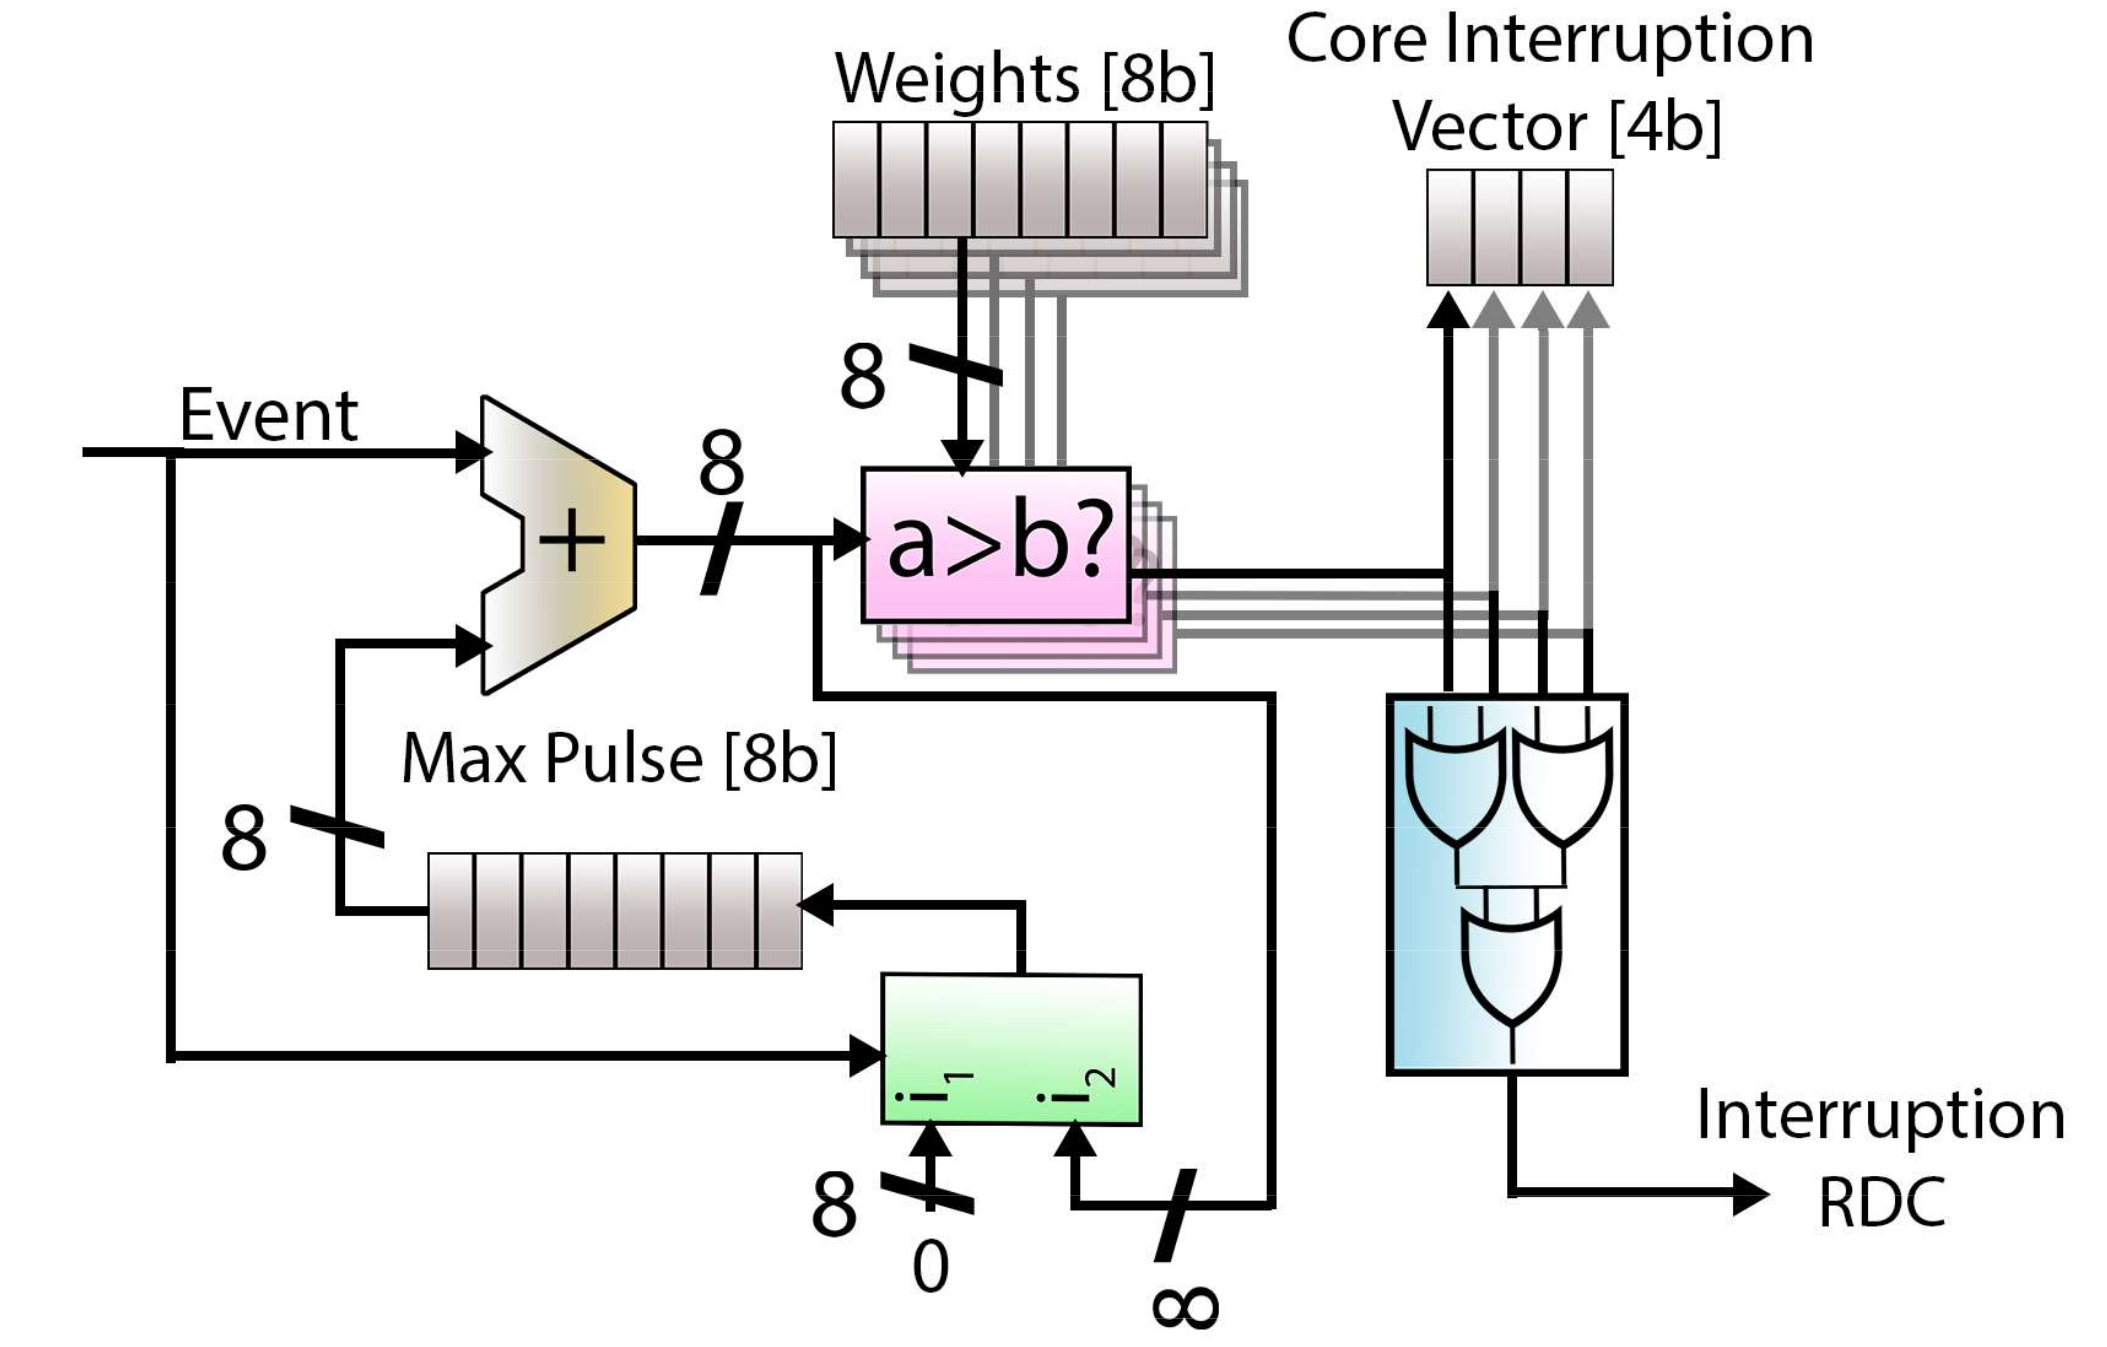
\includegraphics[keepaspectratio,scale=0.15]{img/bd_RDC.png}
	\caption{Block diagram RDC mechanism.}
	\label{fig:blk_RDC}
	\end{center}
\end{figure}

The current release provides monitoring for crossbar outputs 0 to 11 for the hexa-core. Note that the amount of registers changes with the amount of cores, and figures and addresses are representative of the 4 core configuration. The weights for each signal are shared with the MCCU and are stored in registers \ref{RDC_weight0}, \ref{RDC_weight1} and \ref{MCCU_weight1_2}. Weights are 8-bit fields.Counters have overflow protection, preventing the count from wrapping over the maximum value.  The maximum value for each event (watermarks), are stored in registers \ref{RDC_water0}, \ref{RDC_water1} and \ref{RDC_water2}.\\
\\
The RDC shares the main configuration register with the MCCU (register \ref{MCCU_cfg_6c}). Through this register, the unit can be reset and enabled through the corresponding fields. Such fields are active high signals. \\
\\
The unit does provide access to the internal interrupt vector (register \ref{RDC_intrv}), but such information is redundant and may be removed in future releases. Given the current watermarks and assigned weights, the events responsible for the interrupt can be identified.
\\
\textit{Weights not configured or with value 0 will not raise interruptions.}
%The RDC interrupt has been routed to AHB interrupt 11.


\begin{register}{H}{RDC interrupt vector}{0x0D4}
	\label{RDC_intrv}
	\regfield{Reserved}{28}{4}{{x}}
	\regfield{Core 5}{1}{3}{{00}}
	\regfield{Core 4}{1}{3}{{00}}
	\regfield{Core 3}{1}{3}{{00}}
	\regfield{Core 2}{1}{2}{{00}}
	\regfield{Core 1}{1}{1}{{00}}
	\regfield{Core 0}{1}{0}{{00}}
	\reglabel{Reset value}\regnewline
\end{register}
\begin{register}{H}{RDC event weights register 0 (shared with MCCU)}{0x0C0}
	\label{RDC_weight0}
	\regfield{Input 3}{8}{24}{{00}}
	\regfield{Input 2}{8}{16}{{00}}
	\regfield{Input 1}{8}{8}{{00}}
	\regfield{Input 0}{8}{0}{{00}}
	\reglabel{Reset value}\regnewline
\end{register}
\begin{register}{H}{RDC event weights register 1 (shared with MCCU)}{0x0C4}
	\label{RDC_weight1}
	\regfield{Input 7}{8}{24}{{00}}
	\regfield{Input 6}{8}{16}{{00}}
	\regfield{Input 5}{8}{8}{{00}}
	\regfield{Input 4}{8}{0}{{00}}
	\reglabel{Reset value}\regnewline
\end{register}
\begin{register}{H}{RDC event weights register 2 (shared with MCCU)}{0x0C8}
	\label{MCCU_weight1_2}
	\regfield{Input 11}{8}{24}{{00}}
	\regfield{Input 10}{8}{16}{{00}}
	\regfield{Input 9}{8}{8}{{00}}
	\regfield{Input 8}{8}{0}{{00}}
	\reglabel{Reset value}\regnewline
\end{register}


\begin{register}{H}{RDC watermark register 0}{0x0D8}
	\label{RDC_water0}
	\regfield{Input 3}{8}{24}{{00}}
	\regfield{Input 2}{8}{16}{{00}}
	\regfield{Input 1}{8}{8}{{00}}
	\regfield{Input 0}{8}{0}{{00}}
	\reglabel{Reset value}\regnewline
\end{register}


\begin{register}{H}{RDC watermark register 1}{0x0DC}
	\label{RDC_water1}
	\regfield{Input 7}{8}{24}{{00}}
	\regfield{Input 6}{8}{16}{{00}}
	\regfield{Input 5}{8}{8}{{00}}
	\regfield{Input 4}{8}{0}{{00}}
	\reglabel{Reset value}\regnewline
\end{register}

\begin{register}{H}{RDC watermark register 2}{0x0E0}
	\label{RDC_water2}
	\regfield{Input 11}{8}{24}{{00}}
	\regfield{Input 10}{8}{16}{{00}}
	\regfield{Input 9}{8}{8}{{00}}
	\regfield{Input 8}{8}{0}{{00}}
	\reglabel{Reset value}\regnewline
\end{register}


\subsection{Software support}
The unit can be configured by the user at a low level following the description of previous sections and \href{https://gitlab.bsc.es/caos_hw/hdl_ip/bsc_pmu/-/tree/develop/docs}{the documents associated for each unit}. In addition we provide a small bare-metal driver under the \textit{drivers} directory of the SafeSU repository.\\
\\
Currently 3 configurations are provided. \textit{4-core} and \textit{6-core} folders have the driver for default configurations. \textit{6-core-256e} folder has a driver for an hexacore with 256 entries on the crossbar.\\
\\
The drivers are composed of three files.
\begin{itemize}
\item \textit{pmu\_vars.h }: Defines a set of constants with the RTL parameters that generated the unit. Such constants allow the reusing of functions among hardware configurations.
\item\textit{ pmu\_hw.h}: Defines the memory position of the SafeSU within the memory map of the SoC. It also contains the prototypes of each function of the driver.
\item \textit{pmu\_hw.c}: Contains the definition of each of the functions.
\end{itemize}
Given the current development status, the driver is not autogenerated, and \textbf{modifications to the RTL may require manual changes on the previous files}.

%Initialitation (softrware flush)
